% ============================================================
% 问题四：救援任务分区与资源配置优化
% 建议插入 body.tex 中问题三之后、“模型评价与改进”之前
% 图路径按 code/4/output/figures 设置；若目录不同请统一替换。
% ============================================================

% ---------- 问题四最终结果宏 ----------
\newcommand{\QFourUnitNum}{9}
\newcommand{\QFourStrictComponentNum}{1}
\newcommand{\QFourKTwoPartitionNum}{255}
\newcommand{\QFourKThreePartitionNum}{3025}
\newcommand{\QFourTwoRelayMin}{3}
\newcommand{\QFourThreeRelayMin}{4}
\newcommand{\QFourTwoRelayMain}{4}
\newcommand{\QFourThreeRelayMain}{6}
\newcommand{\QFourTwoRelayEnergyMain}{6}
\newcommand{\QFourThreeRelayEnergyMain}{8}
\newcommand{\QFourTwoCopy}{5}
\newcommand{\QFourThreeCopy}{7}
\newcommand{\QFourTwoDeltaEnergy}{2.471}
\newcommand{\QFourThreeDeltaEnergy}{3.918}
\newcommand{\QFourTwoCV}{0.111}
\newcommand{\QFourThreeCV}{0.448}
\newcommand{\QFourTwoZeroTransportNum}{3}
\newcommand{\QFourThreeZeroTransportNum}{1}

\section{问题四：救援任务分区与独立资源配置}
\label{sec:q4}

\subsection{问题分析与总体思路}

问题四不再重新改变问题三得到的货箱组批、服务区访问顺序、运输架次时刻和中继保障关系，
而是在既定联合调度基础上研究：当15个服务区被划分为2个或3个相对独立的任务组后，
各组分别需要配置多少运输无人机、共享电池、中继无人机和中继能源组件，
以及禁止跨组共享后会产生多大的资源冗余和库存缺口。
因此，本问属于\textbf{固定任务时刻表下的分区与资源再配置问题}，
而不是对问题三再次进行运输--通信联合优化。

近期多无人机任务分配研究表明，有限资源、任务依赖和通信约束会显著改变任务划分与资源配置结果\cite{q4-park2025,q4-chu2025}；
灾后搜救场景还需同时关注任务时效、能源与物资资源的协同利用\cite{q4-zhang2026}。
结合本题一个中继架次可能同时服务多个运输单元的特点，
本文采用\textbf{中继关联超图+完整枚举+区间资源配置}的求解框架：
首先由多点运输架次构造不可拆分运输单元，
再以实际中继架次为超边描述高阶共享关系；
随后区分严格继承与按组复制两种解释，
在可执行的扩展口径下完整枚举所有2组、3组分区，
并精确核算各组最少实体资源数量。

\begin{figure}[htbp]
    \centering
    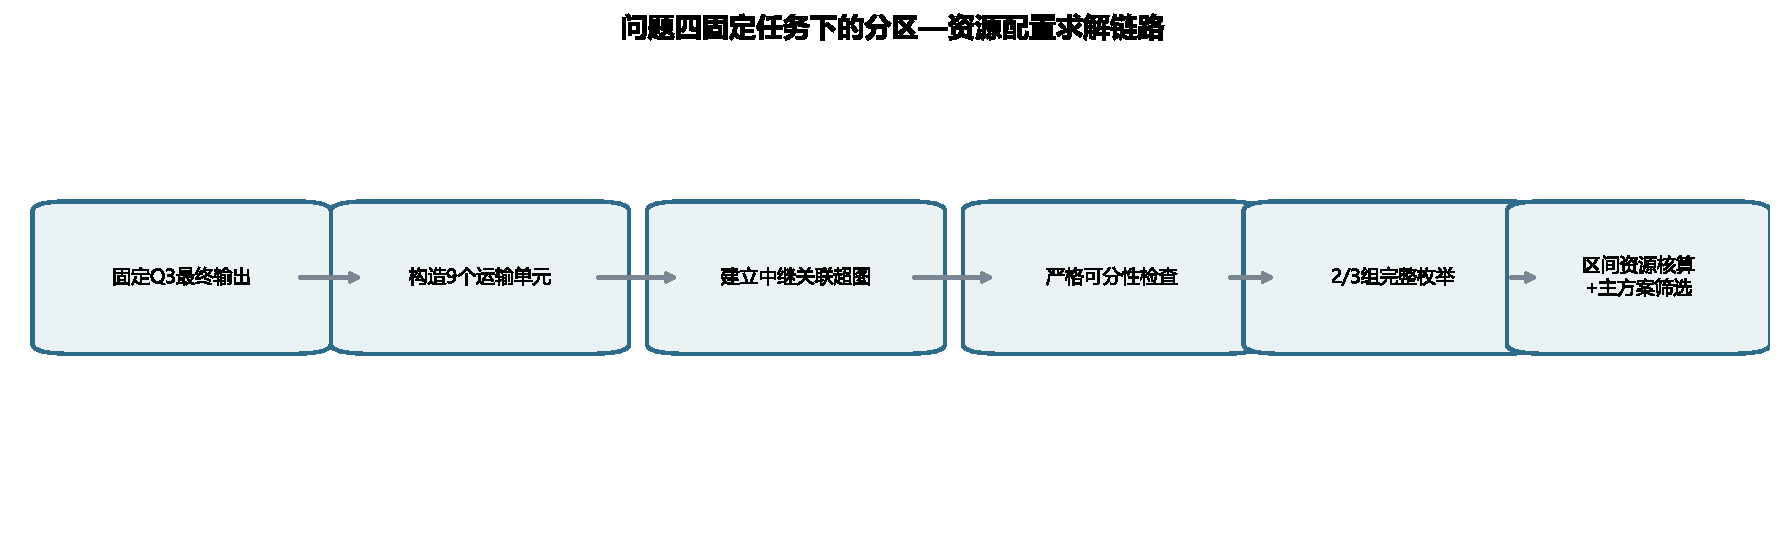
\includegraphics[width=0.96\linewidth]{../../code/4/output/figures/fig_q4_01_solution_flow.pdf}
    \caption{问题四固定任务下的分区--资源配置求解流程}
    \label{fig:q4-flow}
\end{figure}
\FloatBarrier

\subsection{任务不可拆分单元与中继关联超图}

\subsubsection{运输不可拆分单元}

题目要求同一运输架次若访问多个服务区，则这些服务区必须属于同一任务组。
因此，以15个服务区为顶点，对同一运输架次访问的服务区建立等价关系并取传递闭包。
由问题三25个运输架次得到\QFourUnitNum 个不可拆分运输单元：
\begin{equation}
\begin{aligned}
U_1&=\{S001,S013\}, & U_2&=\{S002\}, & U_3&=\{S003\},\\
U_4&=\{S004\}, & U_5&=\{S005,S011\}, & U_6&=\{S006,S007\},\\
U_7&=\{S008,S015\}, & U_8&=\{S009,S012\}, & U_9&=\{S010,S014\}.
\end{aligned}
\label{eq:q4-units}
\end{equation}

上述压缩直接继承问题三的实际运输路线，不依据地理距离重新合并服务区。
因此，即使两个服务区空间上接近，只要未被同一既定运输架次绑定，仍可在问题四中分别划组；
反之，同一多点运输架次中的服务区即使空间跨度较大，也不得拆分。

\subsubsection{中继关联超图}

普通图的一条边只能连接两个顶点，而问题三中一个中继架次可能同时保障多个运输架次，
进而同时关联多个运输单元。
因此，将运输单元集合记为
\(
\mathcal U=\{U_1,\ldots,U_9\}
\)，
并将每一个实际中继架次 $q$ 定义为一条超边
\begin{equation}
 e_q=\{U_i:\ U_i\text{中的至少一个运输架次实际使用中继 }q\}.
 \label{eq:q4-hyperedge}
\end{equation}
这里的关联关系严格来自问题三输出表 \texttt{Q3\_通信保障} 中实际出现的“运输架次--中继架次”记录，
不使用候选覆盖集合替代实际分配关系。

超图划分中常用超边连通度
\(
\lambda_q=|\Lambda(e_q)|
\)
描述一条超边跨越的分区数，
并以 $\lambda_q-1$ 度量其跨区连接代价\cite{q4-eyubov2025}。
本文不采用 FREIGHT 的流式求解算法，而仅借鉴该超图表示与 connectivity/$\lambda-1$ 指标，
并将其赋予本题明确的物理含义：原中继任务 $q$ 若跨越 $\lambda_q$ 个独立任务组，
则需要增加 $\lambda_q-1$ 个完整中继任务副本。

\begin{figure}[htbp]
    \centering
    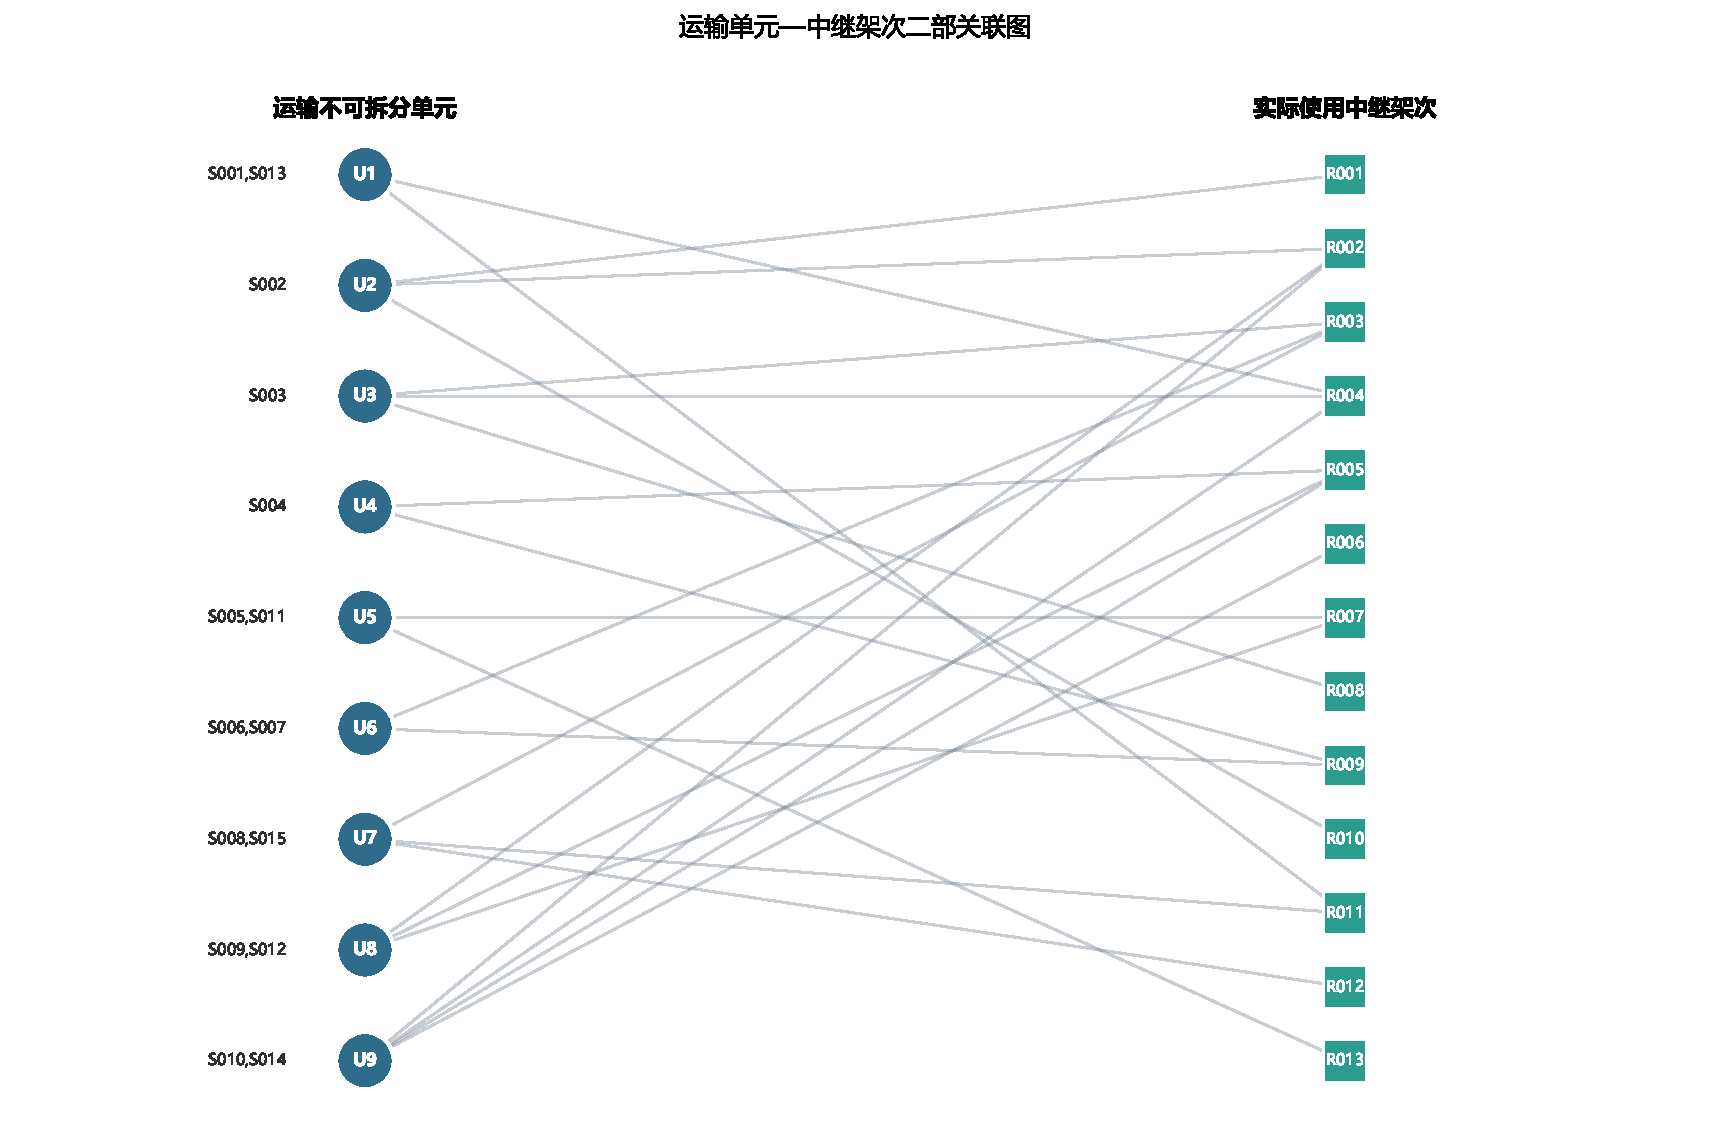
\includegraphics[width=0.96\linewidth]{../../code/4/output/figures/fig_q4_07_unit_relay_bipartite.pdf}
    \caption{运输不可拆分单元与实际中继架次的二部关联图}
    \label{fig:q4-bipartite}
\end{figure}
\FloatBarrier

由图~\ref{fig:q4-bipartite} 可见，多条共享中继超边通过不同运输单元形成传递关联。
将同一中继架次涉及的运输单元视为必须同组，并取传递闭包后，
9个运输单元最终只有 \QFourStrictComponentNum 个连通分量，即全部运输单元被连接为一个整体。
因此，若将“保持中继任务安排及通信保障关系不变”严格解释为
\textbf{原中继架次既不能跨组共享，也不允许复制}，
则2组和3组任务分区均结构性不可行；
这种不可行性来自任务关联结构，而不是简单增加库存即可消除。

\subsection{按组复制中继任务的独立配置模型}

为完成题目要求的2组、3组资源配置比较，
本文进一步采用“中继任务按组完整复制”的独立执行口径：
运输任务保持完全不变；若同一原中继架次服务多个任务组，
则每个涉及该中继的任务组各配置一个独立副本。
副本的悬停经纬度、悬停海拔、开始时刻、建链完成时刻、服务结束时刻、返航时刻及单架次能耗均与问题三原任务一致，
每组对同一原中继任务最多复制一次。
该口径只改变资源归属和中继任务副本数量，不重新优化中继位置与通信时段。

\subsubsection{分区变量与中继复制代价}

设需要划分为 $K$ 个任务组，$K\in\{2,3\}$，定义
\begin{equation}
 x_{ig}=\begin{cases}
 1,&U_i\text{分配至任务组 }g,\\
 0,&\text{否则},
 \end{cases}
 \qquad
 \sum_{g=1}^{K}x_{ig}=1,
 \label{eq:q4-x}
\end{equation}
并要求每个任务组非空。
进一步定义
\begin{equation}
 y_{qg}=\begin{cases}
 1,&\text{任务组 }g\text{中至少有一个运输单元需要中继 }q,\\
 0,&\text{否则}.
 \end{cases}
 \label{eq:q4-y}
\end{equation}
则原中继任务 $q$ 跨越的组数为
\begin{equation}
 \lambda_q=\sum_{g=1}^{K}y_{qg}.
 \label{eq:q4-lambda}
\end{equation}
完整复制口径下新增中继任务副本数为
\begin{equation}
 \boxed{
 N_{\mathrm{copy}}=\sum_q(\lambda_q-1)
 }.
 \label{eq:q4-copy}
\end{equation}
若原中继架次 $q$ 的实际能耗为 $E_q^R$，则新增中继能耗为
\begin{equation}
 \boxed{
 \Delta E_R=\sum_q(\lambda_q-1)E_q^R
 }.
 \label{eq:q4-extra-energy}
\end{equation}
该式直接使用问题三各中继架次的真实能耗，不额外设置缺乏物理依据的统一复制惩罚系数。

\subsubsection{通信链路预算的继承性}

问题四不重新构造通信传播模型，而严格继承问题三已经参数化并逐轨迹采样验证的链路预算。
问题三已将载波频率、发射功率、天线增益、系统损耗、接收灵敏度、衰落裕量和地形遮挡附加损耗用于自由空间损耗与双向链路裕量计算，
并利用30~m DEM 判断地形视距。
记问题三任一链路在时刻 $t$ 的链路裕量为
\begin{equation}
 M_{ab}(t)=L_{ab}^{\max}-L_{ab}(t).
 \label{eq:q4-margin-inherit}
\end{equation}
在问题四中，运输轨迹与时刻不变，中继副本又保持原中继经纬度、海拔及完整服务时段不变，
故同一保障关系对应的端点位置、三维距离、DEM遮挡状态与链路预算参数均不发生变化，
从而有
\begin{equation}
 M_{ab}^{\mathrm{copy}}(t)=M_{ab}^{\mathrm{Q3}}(t).
 \label{eq:q4-margin-equal}
\end{equation}
因此，只要问题三原保障链路满足 $M_{ab}^{\mathrm{Q3}}(t)\ge0$，
其按组完整复制后的单链路通信可用性仍保持不变。
问题四新增约束集中在“各组能否独立配置足够的实体中继资源”，而不是重新改变传播条件。

需要说明的是，问题三通信区间由30~s轨迹采样记录压缩得到，
其中少量导出区间末端可能因“最后采样点+30~s”的记录方式略超过中继服务结束时刻。
问题四构造超图时只使用实际出现的中继编号关联；
资源占用时段则读取中继架次表中的准确开始、返航和充电完成时刻，
因此该导出显示误差不参与资源核算。

\subsubsection{固定时刻表下的最少资源配置}

对每个候选分区，分别提取各任务组的固定运输架次和所需中继任务副本。
对于某类同质资源 $a$，任务 $j$ 的占用时间区间记为 $[s_j,e_{j,a})$。
本文采用以下资源占用口径：
\begin{itemize}
    \item 运输无人机：$[\text{开始},\text{返航})$；
    \item 运输共享电池：$[\text{开始},\text{充电完成})$；
    \item 中继无人机：$[\text{开始},\text{返航}+300\text{s})$；
    \item 中继能源组件：$[\text{开始},\text{充电完成})$。
\end{itemize}
其中A、B、C三种运输机及其共享电池分别建立独立资源池，不能跨型替代。

固定时间区间下，同质资源的最少配置数量等于最大同时占用深度；
按任务开始时刻排序，并优先复用最早释放的资源，可以达到该下界\cite{q4-kleinberg2006}。
因此任务组 $g$ 对资源 $a$ 的最少需求为
\begin{equation}
 \boxed{
 n_{g,a}=\max_t\sum_{j\in\mathcal J_{g,a}}
 \mathbf 1\{s_j\le t<e_{j,a}\}
 }.
 \label{eq:q4-resource-depth}
\end{equation}
程序同时使用最小堆完成实体资源重新编号，
从而不仅得到“至少需要几架/几组资源”，还可以给出每个新编号具体承担哪些固定任务，
并再次检查同一资源是否存在时间冲突。

\subsection{评价指标与完整枚举求解}

\subsubsection{资源规模、冗余与缺口}

设问题三全部固定任务仍允许统一共享资源时的最少需求为 $N_a^{\mathrm{pool}}$，
分为 $K$ 个独立任务组后的总配置需求为
\begin{equation}
 N_a^{(K)}=\sum_{g=1}^{K}n_{g,a}.
 \label{eq:q4-total-resource}
\end{equation}
由任务分区造成的资源冗余定义为
\begin{equation}
 R_a^{(K)}=N_a^{(K)}-N_a^{\mathrm{pool}},
 \label{eq:q4-redundancy}
\end{equation}
相对题目现有库存 $I_a$ 的资源缺口为
\begin{equation}
 D_a^{(K)}=\max\{0,N_a^{(K)}-I_a\}.
 \label{eq:q4-shortage}
\end{equation}
不同机型和不同能源资源的缺口分别报告，
不使用“A型电池富余抵消中继无人机短缺”之类跨资源折算。

\subsubsection{组间工作量均衡}

为避免仅按服务区数量判断任务量，定义任务组 $g$ 的固定运输工作量为
\begin{equation}
 W_g^T=\sum_{r\in\mathcal R_g^T}(f_r-s_r),
 \label{eq:q4-workload}
\end{equation}
并以变异系数衡量组间均衡程度：
\begin{equation}
 CV_T=\frac{
 \sqrt{\frac{1}{K}\sum_{g=1}^{K}(W_g^T-\bar W^T)^2}
 }{\bar W^T}.
 \label{eq:q4-cv}
\end{equation}
同时在详细结果中保留服务区数、货箱数、运输架次数和中继架次数作为解释指标。

\subsubsection{完整枚举与无权重分层筛选}

由于仅有9个不可拆分运输单元，
将其无标签地划分为2组和3组的方案数分别为
\begin{equation}
 S(9,2)=\QFourKTwoPartitionNum,
 \qquad
 S(9,3)=\QFourKThreePartitionNum,
 \label{eq:q4-stirling}
\end{equation}
其中 $S(n,k)$ 为第二类 Stirling 数。
因此本题无需继续使用随机启发式算法；
完整枚举能够逐一计算每个方案的资源需求、复制代价和均衡性，
得到确定、可复现的全体候选集合。
对于大规模超图划分，可借鉴多层并行超图划分等方法\cite{q4-krause2025}，
但本题规模下完整枚举更直接可靠。

由于题目未提供不同设备的采购价格或统一价值系数，
本文不将“1架中继无人机、1组电池、工作量偏差”等强行线性加权，
而采用如下分层筛选规则：
\begin{enumerate}[label=(\arabic*),leftmargin=3em]
    \item 优先保留运输无人机和运输电池均不需要新增的方案；
    \item 在上述方案中优先减少中继无人机总配置；
    \item 再减少中继能源组件配置和中继任务新增副本数；
    \item 在资源规模相近时，选取运输工作量 $CV_T$ 较小的方案；
    \item 同时保留理论最少中继资源方案与Pareto候选，用于说明资源--均衡权衡。
\end{enumerate}

\subsection{求解结果与分析}

\subsubsection{严格继承情景的可分性结论}

根据实际通信保障关系构造的超图将9个运输不可拆分单元连接成单一连通整体。
因此，在“原中继架次不可复制、各类资源不得跨组调配”的严格口径下，
不存在合法的2组或3组独立执行方案。
这说明问题四的关键矛盾不是服务区地理位置本身，
而是问题三为提高中继利用率形成的跨运输单元共享关系。

\subsubsection{两组主方案}

在允许按组完整复制原中继任务后，K=2共有 \QFourKTwoPartitionNum 个无标签候选分区，
其中不存在所有资源均在现有库存内的方案；
但有 \QFourTwoZeroTransportNum 个方案可保持运输侧完全零增配。
按上述分层规则得到的主方案如表~\ref{tab:q4-k2}。

\begin{table}[htbp]
\centering
\caption{K=2 主方案任务分区与独立资源配置}
\label{tab:q4-k2}
\resizebox{\linewidth}{!}{
\begin{tabular}{clcccccccc}
\toprule
组 & 服务区 & A机 & B机 & C机 & A电池 & B电池 & C电池 & 中继机 & 中继能源\\
\midrule
1 & S001,S003,S005,S006,S007,S011,S013 & 2 & 1 & 1 & 2 & 1 & 2 & 2 & 2\\
2 & S002,S004,S008,S009,S010,S012,S014,S015 & 2 & 1 & 1 & 4 & 1 & 2 & 2 & 4\\
\midrule
合计 & -- & 4 & 2 & 2 & 6 & 2 & 4 & 4 & 6\\
\bottomrule
\end{tabular}}
\end{table}
\FloatBarrier

该方案仅在通信侧产生库存缺口：现有2架中继无人机需要增加2架，
而6组中继能源组件恰好能够满足独立配置要求；
A、B、C三类运输无人机及运输电池均无需新增。
该方案需要新增 \QFourTwoCopy 个中继任务副本，
对应新增中继能耗约 \QFourTwoDeltaEnergy~kWh，
运输工作量变异系数为 \QFourTwoCV。

值得区分的是，如果只追求“中继无人机总配置最少”而不要求运输侧零增配和较好均衡，
K=2 的理论下界可达到 \QFourTwoRelayMin 架；
本文提交方案配置 \QFourTwoRelayMain 架中继无人机，
体现了通信资源规模与运输侧独立配置、工作量均衡之间的权衡。

\begin{figure}[htbp]
    \centering
    \includegraphics[width=0.94\linewidth]{../../code/4/output/figures/fig_q4_61_K2_geo_routes_relays.pdf}
    \caption{K=2 主方案运输路线、任务分区与中继复制空间关系}
    \label{fig:q4-k2-geo}
\end{figure}
\FloatBarrier

图~\ref{fig:q4-k2-geo} 在30~m DEM背景上叠加了问题三固定运输路线、服务区分组和各组需要执行的原中继悬停任务。
可见问题四并未按照简单的地理聚类划分服务区，
而是在满足既有多点运输架次不可拆分的前提下，
兼顾共享中继切割代价和资源均衡。

\subsubsection{三组主方案}

K=3共有 \QFourKThreePartitionNum 个无标签候选分区，
同样不存在现有库存全部满足的方案；
仅有 \QFourThreeZeroTransportNum 个方案能够保持运输侧完全零增配，
因此该方案在运输资源约束下实际上具有唯一性。
最终配置见表~\ref{tab:q4-k3}。

\begin{table}[htbp]
\centering
\caption{K=3 主方案任务分区与独立资源配置}
\label{tab:q4-k3}
\resizebox{\linewidth}{!}{
\begin{tabular}{clcccccccc}
\toprule
组 & 服务区 & A机 & B机 & C机 & A电池 & B电池 & C电池 & 中继机 & 中继能源\\
\midrule
1 & S001,S003,S005,S006,S007,S011,S013 & 2 & 1 & 1 & 2 & 1 & 2 & 2 & 2\\
2 & S002,S004,S008,S009,S012,S015 & 1 & 1 & 1 & 2 & 1 & 2 & 2 & 3\\
3 & S010,S014 & 1 & 0 & 0 & 2 & 0 & 0 & 2 & 3\\
\midrule
合计 & -- & 4 & 2 & 2 & 6 & 2 & 4 & 6 & 8\\
\bottomrule
\end{tabular}}
\end{table}
\FloatBarrier

三组方案仍不需要新增任何运输无人机或运输电池，
但中继无人机需求增至 \QFourThreeRelayMain 架，
相对现有2架形成4架缺口；
中继能源组件需求增至 \QFourThreeRelayEnergyMain 组，
相对现有6组形成2组缺口。
同时需要新增 \QFourThreeCopy 个中继任务副本，
新增中继能耗约 \QFourThreeDeltaEnergy~kWh，
运输工作量变异系数上升至 \QFourThreeCV。
若只追求中继数量，下界可达到 \QFourThreeRelayMin 架，
但对应分区不能同时满足本文的运输侧零增配优先规则。

\begin{figure}[htbp]
    \centering
    \includegraphics[width=0.94\linewidth]{../../code/4/output/figures/fig_q4_62_K3_geo_routes_relays.pdf}
    \caption{K=3 主方案运输路线、任务分区与中继复制空间关系}
    \label{fig:q4-k3-geo}
\end{figure}
\FloatBarrier

\subsubsection{两种分区方式的资源与均衡比较}

固定问题三全部任务统一共享资源时，按时间区间重新分配得到的最少需求为：
A、B、C型运输无人机分别4、2、2架，
A、B、C型共享电池分别6、2、4组，
中继无人机2架，中继能源组件4组。
与现有库存相比，B型电池和中继能源组件存在一定共享冗余，
说明问题三原始资源编号的使用数量不等于固定时刻表下的理论最少数量。

\begin{table}[htbp]
\centering
\caption{统一共享、2组和3组独立配置的资源需求比较}
\label{tab:q4-resource-compare}
\resizebox{\linewidth}{!}{
\begin{tabular}{lcccccc}
\toprule
资源类别 & 统一共享最少需求 & 现有库存 & K=2需求 & K=2缺口 & K=3需求 & K=3缺口\\
\midrule
A型运输无人机 & 4 & 4 & 4 & 0 & 4 & 0\\
B型运输无人机 & 2 & 2 & 2 & 0 & 2 & 0\\
C型运输无人机 & 2 & 2 & 2 & 0 & 2 & 0\\
A型共享电池 & 6 & 6 & 6 & 0 & 6 & 0\\
B型共享电池 & 2 & 4 & 2 & 0 & 2 & 0\\
C型共享电池 & 4 & 4 & 4 & 0 & 4 & 0\\
中继无人机 & 2 & 2 & 4 & 2 & 6 & 4\\
中继能源组件 & 4 & 6 & 6 & 0 & 8 & 2\\
\bottomrule
\end{tabular}}
\end{table}
\FloatBarrier

表~\ref{tab:q4-resource-compare} 表明，分区造成的主要增配压力集中在通信侧。
从2组进一步划分为3组后，运输资源总需求没有增加，
但中继无人机由4架升至6架，中继能源组件由6组升至8组。
其原因是任务组越多，原问题三中能够跨运输任务共享的中继架次越容易被切开，
相同悬停位置和服务时段必须由不同任务组各自配置实体资源执行。

\begin{figure}[htbp]
    \centering
    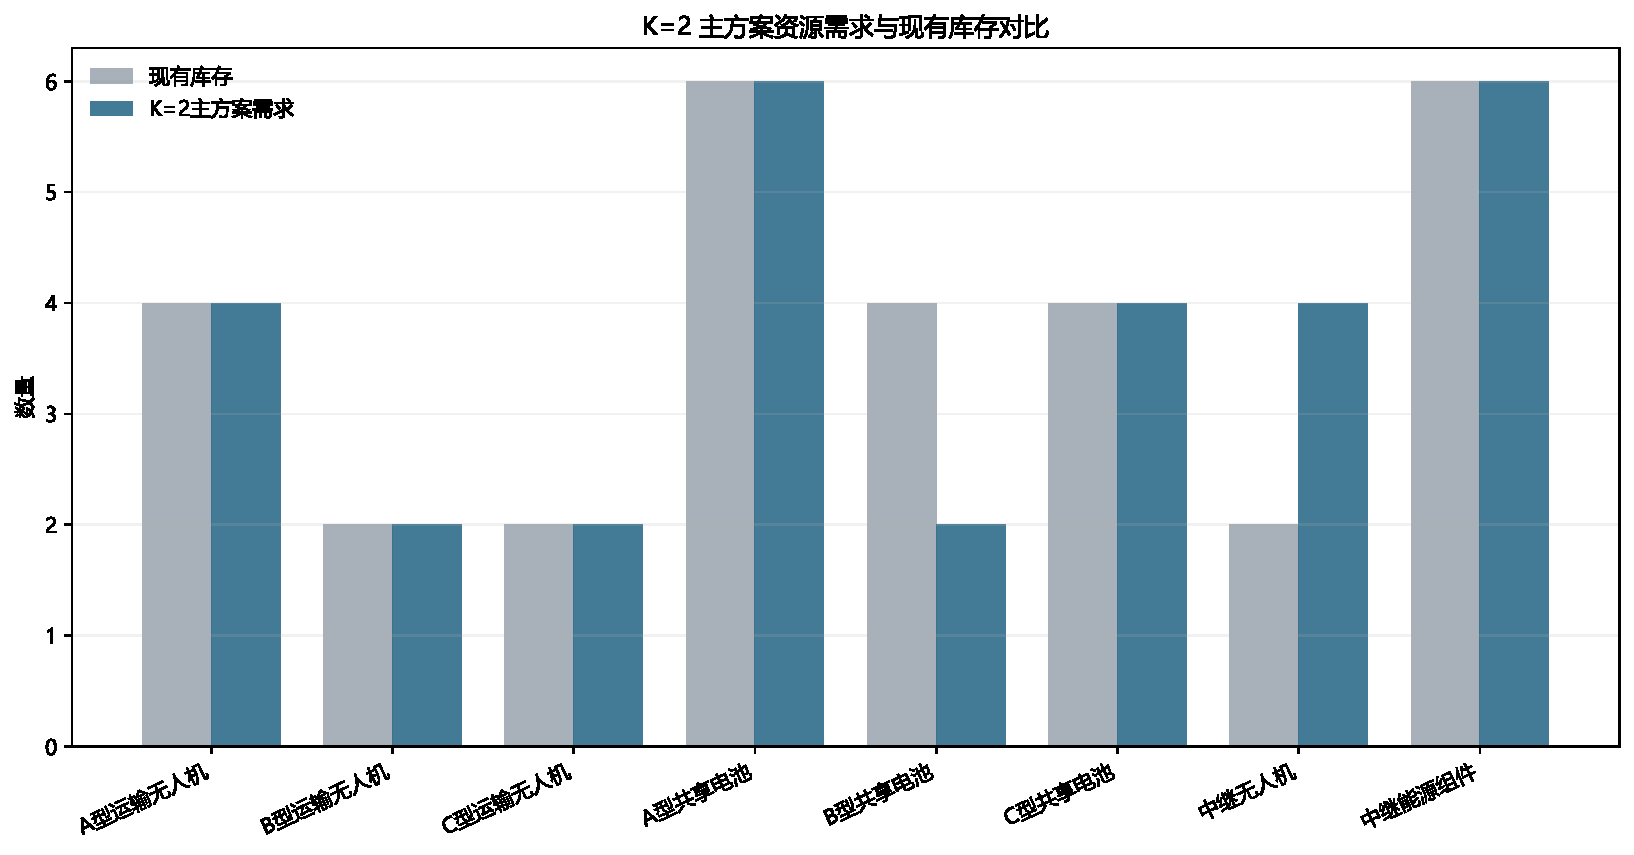
\includegraphics[width=0.88\linewidth]{../../code/4/output/figures/fig_q4_26_K2_resource_vs_stock.pdf}
    \caption{K=2 主方案资源需求与现有库存对比}
    \label{fig:q4-k2-resource}
\end{figure}
\FloatBarrier

\begin{figure}[htbp]
    \centering
    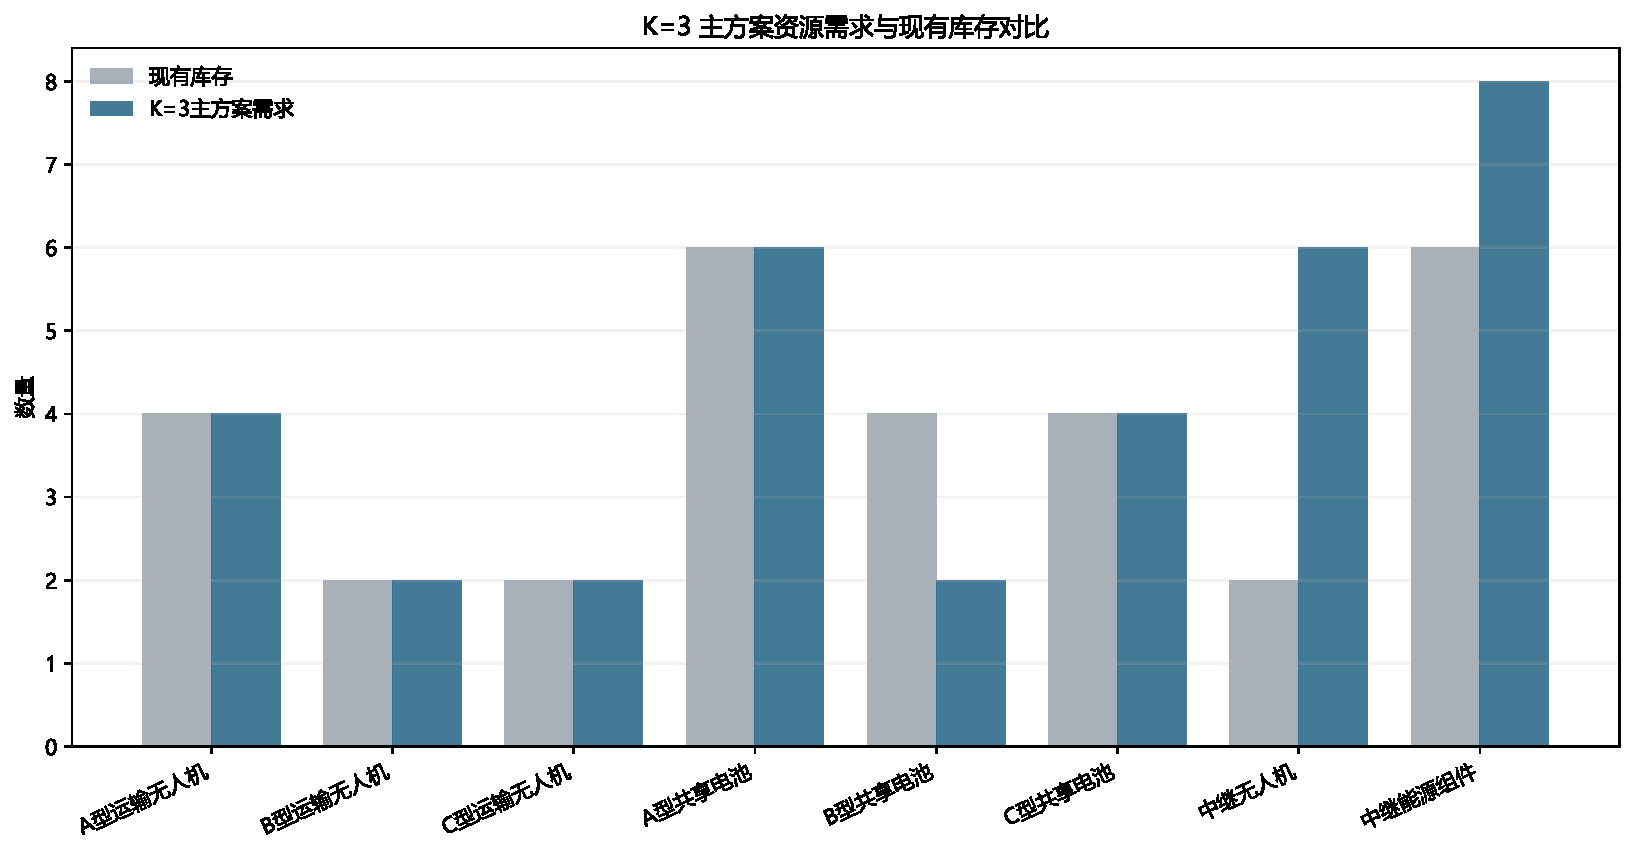
\includegraphics[width=0.88\linewidth]{../../code/4/output/figures/fig_q4_27_K3_resource_vs_stock.pdf}
    \caption{K=3 主方案资源需求与现有库存对比}
    \label{fig:q4-k3-resource}
\end{figure}
\FloatBarrier

完整枚举还揭示了中继共享代价与工作量均衡之间的明显权衡。
图~\ref{fig:q4-k2-tradeoff} 和图~\ref{fig:q4-k3-tradeoff} 中每个点分别对应一个完整候选分区；
横轴为中继新增副本数，纵轴为运输工作量变异系数。
减少中继超边切割通常有利于降低通信资源需求，
但并不必然得到最均衡的运输工作量，
因此本文没有采用单一地理聚类或单一通信资源最小化作为最终选择标准。

\begin{figure}[htbp]
    \centering
    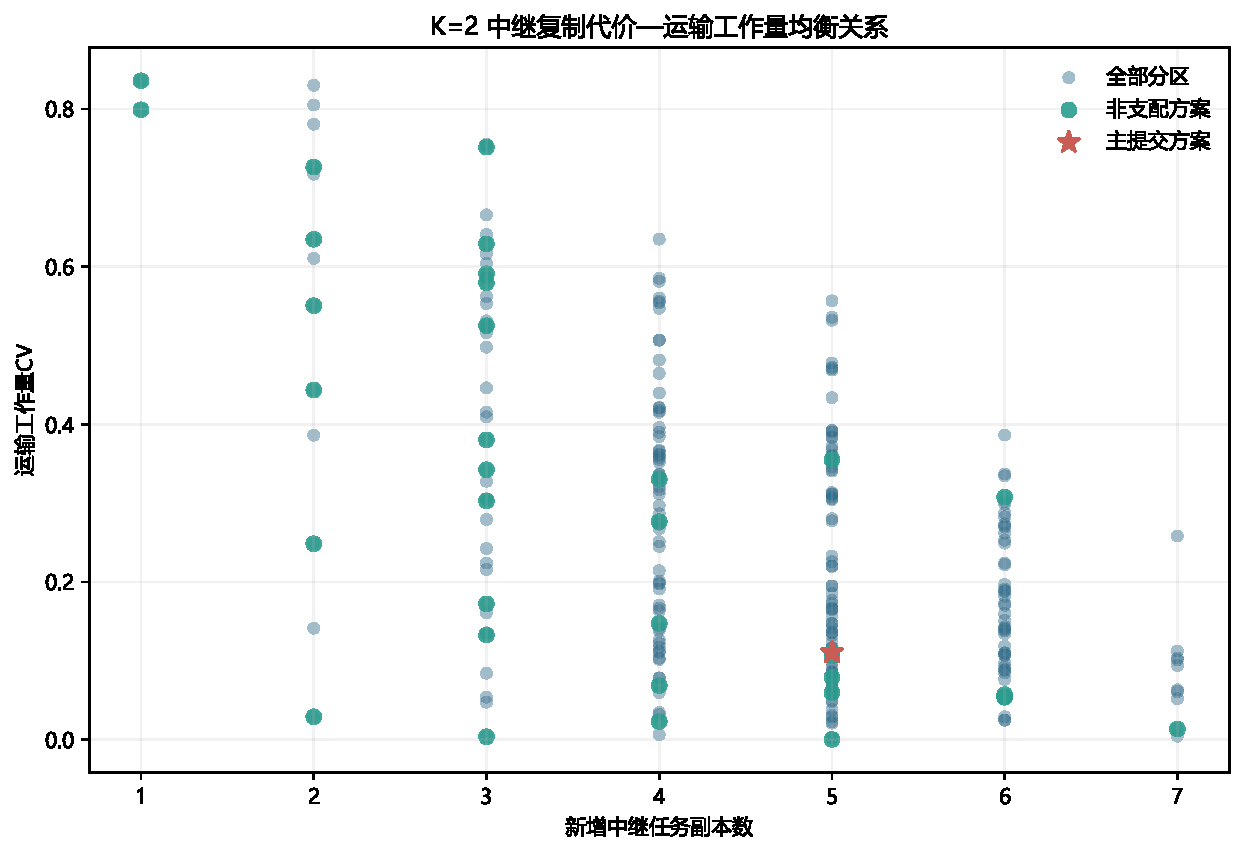
\includegraphics[width=0.82\linewidth]{../../code/4/output/figures/fig_q4_18_K2_copy_balance_scatter.pdf}
    \caption{K=2 中继复制代价与运输工作量均衡关系}
    \label{fig:q4-k2-tradeoff}
\end{figure}
\FloatBarrier

\begin{figure}[htbp]
    \centering
    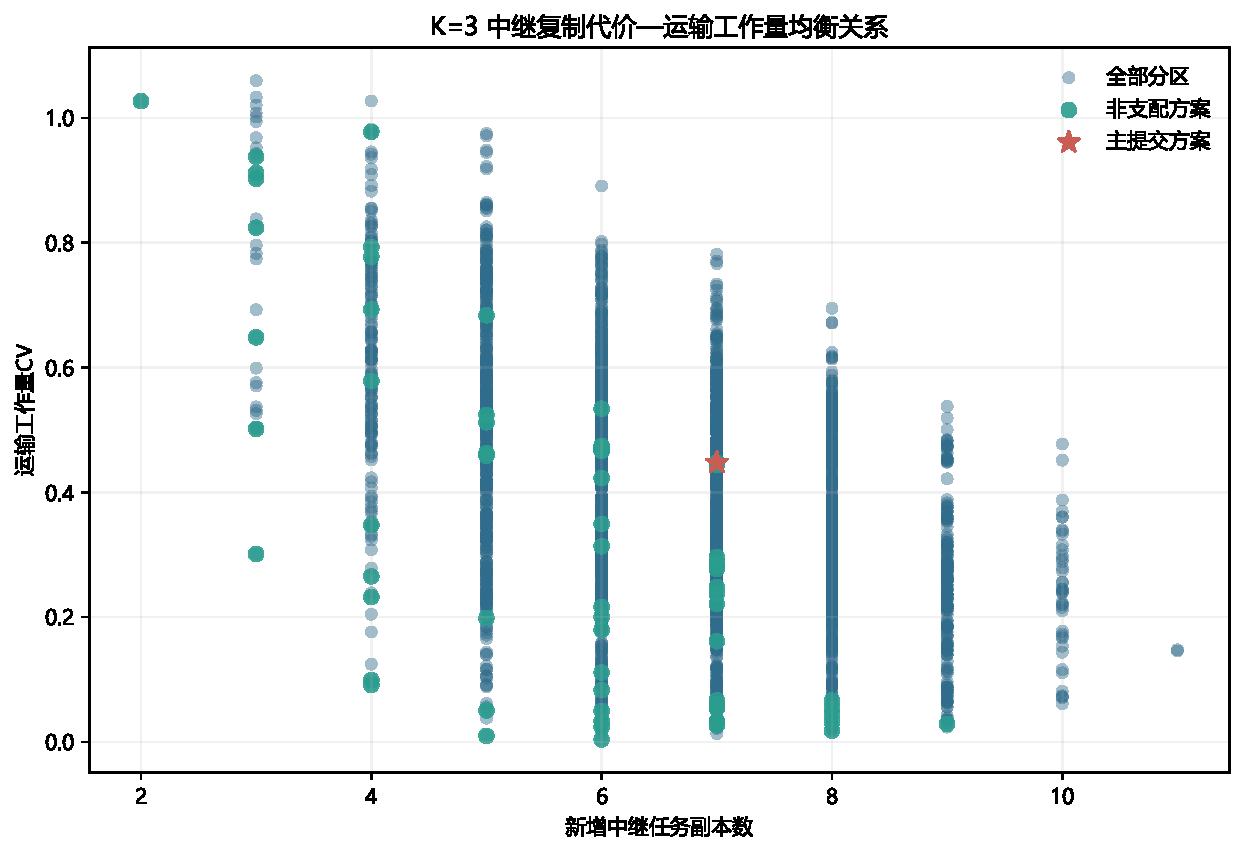
\includegraphics[width=0.82\linewidth]{../../code/4/output/figures/fig_q4_19_K3_copy_balance_scatter.pdf}
    \caption{K=3 中继复制代价与运输工作量均衡关系}
    \label{fig:q4-k3-tradeoff}
\end{figure}
\FloatBarrier

综合来看，2组方案的运输工作量 $CV_T=\QFourTwoCV$，
且仅需新增2架中继无人机；
3组方案的 $CV_T=\QFourThreeCV$，
同时需要新增4架中继无人机和2组中继能源组件。
因此，分成更多独立任务组虽然增强了组织上的独立性，
但会显著损失问题三通过共享中继形成的资源复用优势。
该结论是在固定问题三联合调度、采用完整中继任务复制且禁止跨组调配的口径下得到，
不推广为对所有重新调度方案的一般结论。

\subsection{方案可行性与结果审计}

为保证问题四输出能够直接用于结果提交，程序对最终2组和3组主方案执行以下审计：
\begin{enumerate}[label=(\arabic*),leftmargin=3em]
    \item 每个服务区恰好属于一个任务组，且每组非空；
    \item 同一问题三运输架次访问的多个服务区均位于同一任务组；
    \item 各组运输架次的机型、访问顺序、开始/返航时刻和能耗均与问题三保持一致；
    \item 每个原中继任务在一个任务组内最多建立一个副本，副本位置、高度和完整时段不变；
    \item 按式~\eqref{eq:q4-resource-depth} 重新分配组内实体资源后，同一运输无人机、电池、中继无人机和能源组件均不存在时间重叠；
    \item 中继无人机返航后计入300~s周转时间，能源组件在再次投入任务前必须完成充电；
    \item 问题三已通过链路预算验证的通信关系在副本中保持相同几何和参数，因此通信可用性继承成立；
    \item 最终提交表中的资源数量与程序重新编号后的最大并发占用数一致。
\end{enumerate}

最终程序将2组和3组共5个任务组的配置结果自动写入
\texttt{结果提交模板.xlsx} 的 \texttt{Q4\_分区配置} 工作表，
同时输出全部 \QFourKTwoPartitionNum+\QFourKThreePartitionNum 个候选分区的评价结果、
Pareto候选、组内实体资源重新编号明细、严格不可分证据、资源缺口分析和图形化审计结果。

本问采用完整枚举，因此在\textbf{固定问题三任务、给定中继复制口径和既定分层筛选规则}下，
候选空间被完全遍历；
不同于问题二、问题三的启发式搜索，
这里不存在因随机种子或迭代次数不足而漏掉枚举候选的问题。
但按组复制中继任务属于为满足独立执行要求引入的建模解释，
若实际组织规则明确禁止任何形式的中继任务复制，则应采用前述严格情景结论：2组和3组均无法由当前问题三方案直接实现。

\subsection{程序输出与图表体系}

问题四程序 \texttt{q4\_solver\_v2\_geo.py} 直接读取问题三最终详细结果、
调度中心与服务区坐标、30~m DEM及结果提交模板。
除正式回填文件外，程序还输出完整分区CSV、详细结果Excel、资源重新编号表、审计报告、正文结果宏和参考文献条目。
在可读取节点坐标和DEM时，程序额外生成真实地理分区、固定运输路线、中继悬停点和逐任务组空间执行图。

为避免仅围绕正文选图而丢失诊断信息，程序对求解流程中的结构、分布、资源、均衡、时序和地理结果尽可能进行可视化，
并自动生成独立的 \texttt{Q4\_图表说明.tex}，逐图说明其内容、解释意义和正文使用建议。
正文仅选取最能支撑模型与结论的图，其余图可用于附录、答辩或结果复核。
